\chapter{Evaluation}
\label{chap:evaluation}
Biohadoops purpose is to facilitate the implementation of parallel algorithms on Hadoop. It is expected that the execution time of an algorithm reduces if it is parallelized (assuming the algorithm is suitable for parallelization). That means the speedup increases when computational resources are added. To verify this assumption, two bio-inspired optimization algorithms are parallelized using Biohadoop. Their parallel parts are executed on Biohadoop workers. The execution times of the algorithms are measured on a Hadoop cluster. Then, the speedups are calculated based on those execution times. The speedups demonstrate if the algorithm execution times benefit from the parallelization.

The rest of this chapter is structured as follows: section \ref{chap:evaluation:cluster} provides information about the cluster used for the benchmarks. Section \ref{chap:evaluation:testproblems} describes the benchmarked test problems. The benchmark results are presented in section \ref{chap:evaluation:benchmarks} together with a check for their correctness. Section \ref{chap:evaluation:influence} gives a discussion of the most notable factors that influence the execution time. The speedup calculations can be found in section \ref{chap:evaluation:speedup}. Finally, section \ref{chap:evaluation:comparison} compares the execution times of Biohadoop parallelellized algorithms to their standalone implementations.

\section{Cluster Hardware}
\label{chap:evaluation:cluster}
All benchmarks are performed on a Hadoop cluster with 6 identical computers. Each machine has the following specifications:

\begin{itemize}
  \item Intel Core2 Duo CPU E8200 @ \unit[2.66]{GHz} (2$\times$\unit[2.66]{GHz}, no hyperthreading)
  \item \unit[6]{MB} shared L2 cache, \unit[32]{KB} L1 data cache, \unit[32]{KB} L1 instruction cache
  \item \unit[4]{GB} (2$\times$\unit[2]{GB}) DDR2 RAM @ \unit[667]{MHz}
  \item \unit[64]{Bit} Ubuntu Linux 14.04.1 LTS with kernel 3.13.0-37
\end{itemize}

The computers are directly connected to the same Switch through a 1Gb (Gigabit) Ethernet network.

\section{Test Problems}
\label{chap:evaluation:testproblems}
NSGA-II and a simple GA are the implemented bio-inspired optimization algorithms used for the benchmarks. They can handle different numbers objectives. While NSGA-II is used to solve the MOP in section \ref{chap:evaluation:zdt3}, a simple GA is used to solve the SOP in section \ref{chap:evaluation:tiledmul}.

\subsection{ZDT-3}
\label{chap:evaluation:zdt3}
The first optimization algorithm is NSGA-II, used to find optimal solutions for the Zitzler–Deb–Thiele's function nr. 3 \cite{zitzler2000comparison}. ZDT-3 is part of the well known ZDT family of MOP. It was chosen because of its discontinuous optimal Pareto Front (see figure \ref{fig:zdt3}) that can pose problems to simpler optimization strategies, e.g., gradient based algorithms. The expected outcome is to find an approximation to the optimal Pareto Front.

\begin{figure}
  \centering
  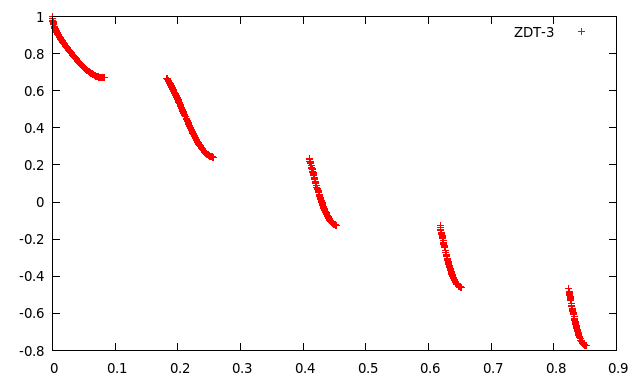
\includegraphics[width=110mm,natwidth=640,natheight=384]{zdt3.png}
  \caption[Optimal Pareto Front for ZDT-3]{Optimal Pareto Front for ZDT-3}
  \label{fig:zdt3}
\end{figure}

The implementation uses Biohadoop workers to create and evaluate the offsprings. Simulated Binary Crossover (SBX) and Parameter based mutation \cite{deb2000efficient} are used for the offspring creation. The fitness is computed using the ZDT-3 function. The selection of the fittest individuals for the next population is based on ranking and crowding distance and is performed on the master.

The ZDT-3 benchmarks are executed with genome sizes of 10, 100, 1000 and 10000. The genome size influences two properties of the ZDT-3 benchmark. First, increasing the number of genomes also increases the computation effort for the workers that generate new offsprings and compute their fitness. This is due to the fact that new individuals are generated using parent genomes and that the ZDT-3 algorithm, used for the fitness computation, loops over all genomes. Second, the genome size influences the amount of data that has to be transferred between the master and the workers. Each worker repeatedly receives two parent individuals and returns an offspring and its computed fitness. The amount of data sent between master and workers is, therefore, related to the gnome size of each individual.

\subsection{Tiled Matrix Multiplication}
\label{chap:evaluation:tiledmul}
The second benchmark implements a GA to solve the SOP for finding optimal tile sizes for the tiled matrix multiplication (TMM). The objective is to minimize the execution time for a matrix multiplication. The expected outcome are tile sizes that minimizes the TMM execution time.

A matrix multiplication can be performed in different ways. The most obvious one is the standard algorithm:
\begin{lstlisting}
for i = 1 to n
  for j = 1 to m
    for k = 1 to l
      C(i,j) = C(i,j) + A(i,k) * B(k,j)
\end{lstlisting}

The matrix multiplication can be improved by loop tiling \cite{wolfe1989more}. The computation is performed on smaller blocks (tiles) of the matrices:
\begin{lstlisting}
for i0 = 1 to n, step blocksize_i
  for j0 = 1 to m, step blocksize_j
    for k0 = 1 to l, step blocksize_k
      for i = i0 to min(i0 + blocksize_i, n)
        for j = j0 to min(j0 + blocksize_j, m)
          for k = k0 to min(k0 + blocksize_k, l)
            C(i,j) = C(i,j) + A(i,k) * B(k,j)
\end{lstlisting}

If the blocks are small enough they fit into the L1 CPU cache which results in a speedup. Tests with a matrix size of 1024$\times$1024 were performed on a single computer of the test cluster to demonstrate the advantages of TMM. Table \ref{table:mm_comparison} shows that suitable tile sizes can reduce the execution times for a tiled matrix multiplication. The results show also that bad tile sizes increase the execution time drastically. Therefore, one needs to find good tile sizes to profit from TMM.

\begin{table}
  \centering
  \caption{Execution times for 1024$\times$1024 matrix multiplications}
  \begin{tabular}{lrr}\toprule[2pt]
    Setting & execution time [s] \\ \midrule
    Standard algorithm & 11.384 \\
    TMM, tile size $i=j=k=1$ & 25.683 & \\
    TMM, tile size $i=j=k=32$ & 2.669 &  \\
  \end{tabular}
  \label{table:mm_comparison}
\end{table}

An optimization algorithm can be used to find the (near) optimal tile sizes for the different loops. In this case, the optimization is done using a GA. The implementation uses Biohadoops workers to create and evaluate an offspring. For the offspring creation, Simulated Binary Crossover (SBX) and Parameter based mutation are used. The fitness is computed as the time it takes to multiply two matrices using a given tile size. The selection of the fittest individuals for the next population is performed on the master.

The TMM benchmarks are executed with matrix sizes of 128$\times$128 and 256$\times$256. The matrix size influences the number of computations that need to be performed for a full matrix multiplication and, therefore, also influences the execution time. In contrast to ZDT-3, the matrix size has no impact on the amount of data transferred between the master and the workers. The matrices are part of the ``initial data'' (see chapter \ref{chap:impl:worker}) and, hence, transferred exactly once to every worker. The task data consists of two parent individuals that are transferred from the master to the workers to create a new offspring and compute its fitness. The data transferred from a worker to the master contains the offspring and its computed fitness value. Each individual consists of its tile sizes for $i$, $j$ and $k$.

\subsection{Settings}
All benchmarks are executed on the cluster described in section \ref{chap:evaluation:cluster}. They have the following settings in common:
\begin{itemize}
  \item The number of iterations is set to 250.
  \item The population size is set to 100.
  \item The distribution index $n_c$ for the SBX crossover is set to 20.
  \item The distribution index $n_m$ for the mutation is set to 20.
  \item The mutation probability for each offspring value is set to $1/n$, i.e., on average one offspring value is mutated.
\end{itemize}

Parallel benchmarks are executed with different problem sizes and different numbers of workers. Standalone sequential benchmarks, used for comparison with the parallel results in section \ref{chap:evaluation:comparison}, are executed with different problem sizes only. It makes no sense to vary the worker size for a sequential benchmark.

% The varying problem size for NSGA-II is defined as the genome size. For TMM it is the matrix size. The number of workers for the parallel benchmarks range from 1 to 15.

% Each benchmark was repeated five times to improve the reliability of the results. This gives a total of 300 benchmark runs for ZDT-3 (4 genome sizes $\times$ 15 worker setting $\times$ 5 repetitions) and 150 benchmark runs for TMM (2 tile sizes $\times$ 15 worker settings $\times$ 5 repetitions).

\section{Biohadoop Benchmarks}
\label{chap:evaluation:benchmarks}
The benchmark results presented in this section show the algorithm execution times (AETs) for the test problems that were parallelized using Biohadoop. It is expected that the AET of a test problem reduces when the number of parallel workers increases.

Before the presentation of the benchmark results, a definition of AET is given for clarification. Then, the benchmark results are presented. Afterwards, the output of the benchmarks, i.e., the optimization results, are checked for correctness.

\subsection{Definition of Algorithm Execution Time}
\label{chap:evaluation:exec-definition}
The full execution time of an algorithm running on top of Biohadoop is composed of the time Biohadoop needs to start up as a Hadoop application and the time spent in the algorithms \texttt{run} method. The time spent in the algorithms \texttt{run} method is from here on defined as AET. Figure \ref{fig:execution-times} demonstrates this concept.

\begin{figure}
  \centering
  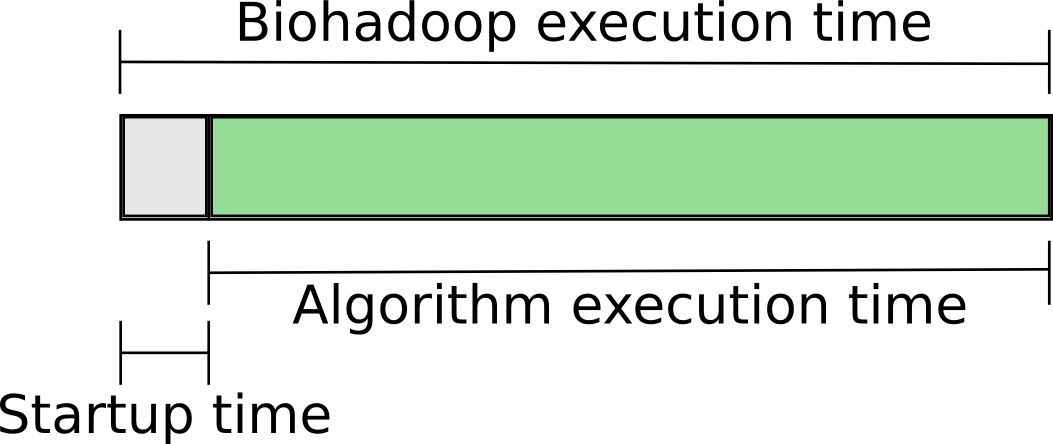
\includegraphics[width=70mm,natwidth=1053,natheight=444]{execution-times.png}
  \caption[Division of Biohadoop execution times]{Biohadoop execution times are composed of start up times and algorithm execution times}
  \label{fig:execution-times}
\end{figure}

The distinction between start up time and AET is made because the main part of the start up time is spent between the application submission to Hadoop and the beginning of its execution. It is not possible to predict when an application is executed by Hadoop as it depends on different factors like the available cluster resources. To minimize the impact of this uncertainty, the following benchmark measurements are based on AET, without the application start up time.

In contrast, the definition of AET for a program that doesn't use Biohadoop is given as the execution time of the Java program. This definition applies to the standalone sequential implementations in section \ref{chap:evaluation:comparison}, which have no Hadoop startup time.

\subsection{Benchmark results}
The results presented in this section reflect the AET for the test problems of section \ref{chap:evaluation:testproblems}. The test problems are parallelized using Biohadoop and its task system. The parallel parts are executed on Biohadoop workers.

The benchmarks are performed with worker sizes ranging from 1 to 15. Each benchmark is repeated five times to improve the reliability of the results. This gives a total of 300 benchmark runs for ZDT-3 (4 genome sizes $\times$ 15 worker setting $\times$ 5 repetitions) and 150 benchmark runs for TMM (2 tile sizes $\times$ 15 worker settings $\times$ 5 repetitions). The AET for the benchmarks are presented in fig. \ref{fig:nsga_250_100_10} to \ref{fig:nsga_250_100_10000} for the ZDT-3 test problem. Fig. \ref{fig:tiledmul_250_100_128x128} and \ref{fig:tiledmul_250_100_256x256} show the results for the TMM benchmarks.

\begin{figure}
  \centering
  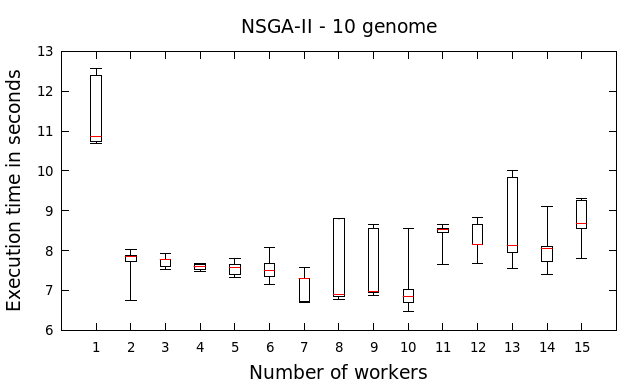
\includegraphics[width=90mm,natwidth=640,natheight=384]{nsgaii_250_100_10.png}
  \caption[ZDT-3 execution times for a genome size of 10]{ZDT-3 execution times for a genome size of 10}
  \label{fig:nsga_250_100_10}
\end{figure}
\begin{figure}
  \centering
  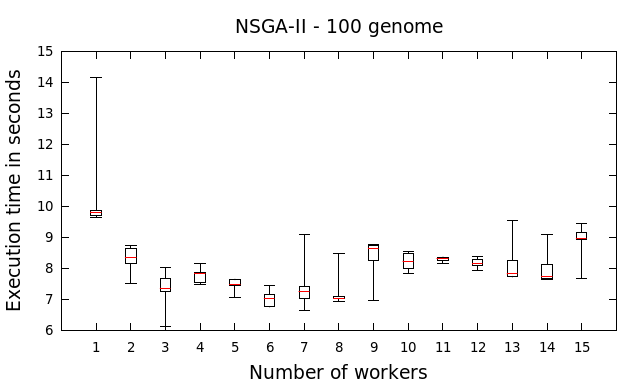
\includegraphics[width=90mm,natwidth=640,natheight=384]{nsgaii_250_100_100.png}
  \caption[ZDT-3 execution times for a genome size of 100]{ZDT-3 execution times for a genome size of 100}
  \label{fig:nsga_250_100_100}
\end{figure}
\begin{figure}
  \centering
  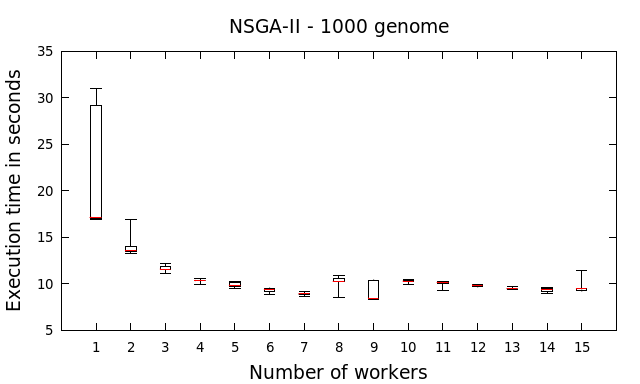
\includegraphics[width=90mm,natwidth=640,natheight=384]{nsgaii_250_100_1000.png}
  \caption[ZDT-3 execution times for a genome size of 1000]{ZDT-3 execution times for a genome size of 1000}
  \label{fig:nsga_250_100_1000}
\end{figure}
\begin{figure}
  \centering
  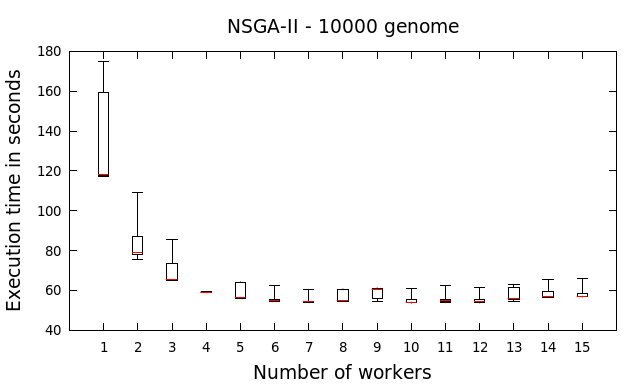
\includegraphics[width=90mm,natwidth=640,natheight=384]{nsgaii_250_100_10000.png}
  \caption[ZDT-3 execution times for a genome size of 10000]{ZDT-3 execution times for a genome size of 10000}
  \label{fig:nsga_250_100_10000}
\end{figure}

\begin{figure}
  \centering
  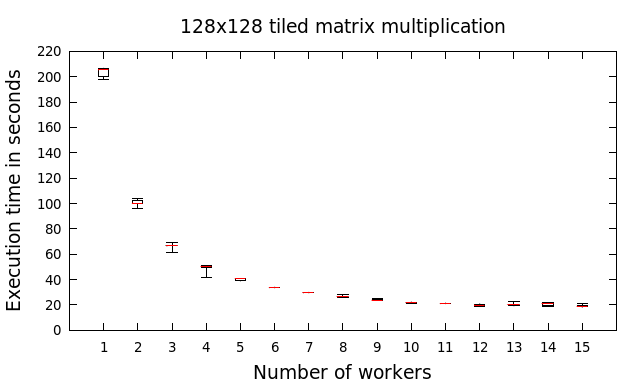
\includegraphics[width=90mm,natwidth=640,natheight=384]{tiledmul_250_100_128x128.png}
  \caption[TMM execution times for a matrix size of 128$\times$128]{TMM execution times for a matrix size of 128$\times$128}
  \label{fig:tiledmul_250_100_128x128}
\end{figure}
\begin{figure}
  \centering
  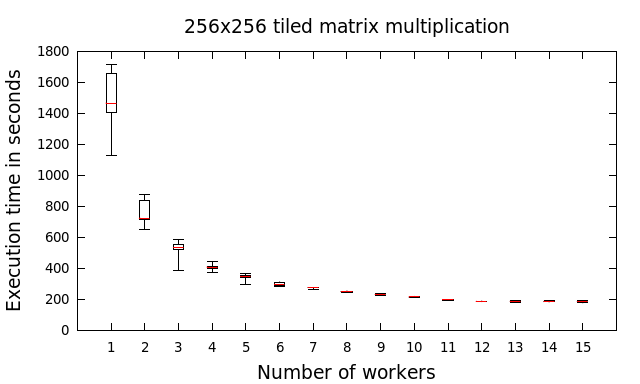
\includegraphics[width=90mm,natwidth=640,natheight=384]{tiledmul_250_100_256x256.png}
  \caption[TMM execution times for a matrix size of 256$\times$256]{TMM execution times for a matrix size of 256$\times$256}
  \label{fig:tiledmul_250_100_256x256}
\end{figure}

All benchmark results demonstrate reduced AETs when the number of workers is increased. The biggest performance gains can be found when stepping from 1 to 2 workers. Further increases of parallel workers show varying success. ZDT-3 benchmarks with 10 and 100 genomes don't seem to profit from more than 2 workers. The performance for genome sizes of 1000 and 10000 increases in the best case until 8 - 9 workers, although, the performance gains are very small. The TMM benchmarks on the other hand show remarkable AET decreases when the number of workers is increased up to 12 workers.

At this point a more in-depth discussion of the benchmark results is put back on purpose, it can be found in section \ref{chap:evaluation:influence} and \ref{chap:evaluation:speedup}. The correctness of the optimization results must be verified first, otherwise, the test problems could execute arbitrary computations and the benchmarks would be meaningless.

\subsection{Correctness of ZDT-3 results}
In the case of ZDT-3 the task was to find an approximation to the optimal Pareto Front (OPF). The computed Pareto Fronts (CPF) are compared to the OPF using the Hypervolume (HV) indicator \cite{zitzler1999multiobjective}. Table \ref{table:hypervolume} gives the results for the indicator, where the HV is computed as the median over all benchmarks for a given genome size. Higher HV values indicate a better CPF.

\begin{table}
  \centering
  \caption{Hypervolume results for ZDT-3 benchmarks}
  \begin{tabular}{lrrrr}\toprule[2pt]
    Test Problem & Hypervolume \\ \midrule
    NSGA-II, 10 genomes & 0.515 \\
    NSGA-II, 100 genomes & 0.458 \\
    NSGA-II, 1000 genomes & 0.340 \\
    NSGA-II, 10000 genomes & 0.330 \\
  \end{tabular}
  \label{table:hypervolume}
\end{table}

One can see that HV decreases with the number of genomes. It is well known that ZDT-3 optimization is harder the larger the genome is. 10 genomes produce the best results with HV = 0.515. Manual comparison of a CPF (randomly chosen from the results with 10 genomes) show high similarities with OPF, as can be seen in fig. \ref{fig:pf-comparison}. It is therefore concluded that the ZDT-3 optimization results are correct.

\begin{figure}
  \centering
  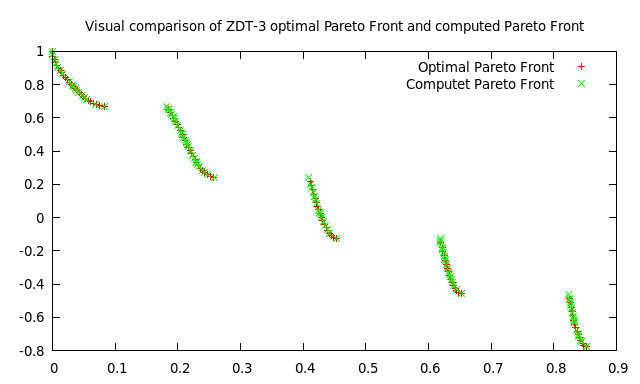
\includegraphics[width=110mm,natwidth=640,natheight=384]{pf-comparison.png}
  \caption[Comparison of optimal and computed PF for ZDT-3]{Visual comparison of ZDT-3 optimal Pareto Front and computed Pareto Front}
  \label{fig:pf-comparison}
\end{figure}

\subsection{Correctness of TMM results}
The goal of TMM optimization was to find tile sizes that reduce the computation time for a tiled matrix multiplication. Other than expected, the found tile sizes follow no recognizable pattern. The explanation is that the solution space is shallow which makes most solutions almost equally well suited. The exception are very small tile sizes with values less than 4.

The TMM optimization results were checked by executing a matrix multiplication with the optimized tile sizes and comparing the results to the execution time of the simple matrix multiplication (SMM). The results were twofold.

For 128$\times$128 matrix sizes, SMMs were faster by \unit[10]{\%} to \unit[15]{\%}. The reason is, that the additional nested loops of TMM and the consequent increased overhead is higher than the performance gain. Another reason is that 128$\times$128 matrices are small enough that sufficient parts of it fit into the L1 CPU caches to profit from the fast access rates.

In the case of 256$\times$256 benchmarks, all TMM executions were faster compared to the SMM by \unit[20]{\%} to \unit[30]{\%}. Additional experiments with larger matrices show that the performance gap between SMM and TMM increases with the matrix size. For example, 512$\times$512 matrix sizes provided about \unit[50]{\%} better performance for TMM. 1024$\times$1024 matrix sizes have about \unit[400]{\%} better performance. Again, the conclusion is that TMM benchmarks produce correct outputs.

\section{Performance Influencing Factors}
\label{chap:evaluation:influence}
Looking at the details of the benchmark results (presented in fig. \ref{fig:nsga_250_100_10} to \ref{fig:tiledmul_250_100_256x256}) two strange behaviours can be observed that need explanation. First, the AET for a benchmark with given setting (e.g. ZDT-3, 100 genomes, one worker) varies by a large amount. This is due to the influence of YARN, discussed in section \ref{chap:evaluation:influence-yarn}. Second, ZDT-3 benchmarks for genome sizes of 10 and 100 experience AET reductions only up to 2 parallel workers, although the cluster provides more resources. The reason for this has been found to be the CPU saturation on Biohadoops master, discussed in section \ref{chap:evaluation:influence-cpu}. Other hard- and software influences on the benchmark results are summarized in section \ref{chap:evaluation:influence-other}. Their impact was not quantified.

It is difficult and a lot of work to find the reasons for performance degradations and strange phenomenas. This is especially true for a distributed environment like Hadoop. Further research could therefore focus on the development of distributed tracing and profiling tools, perhaps adapted to Hadoop. This would greatly simplify performance and bottleneck evaluations. Since Hadoop gains a lot of attraction also in business, it would be a good chance to bridge the gap between science and business.

\subsection{Influence of YARN}
\label{chap:evaluation:influence-yarn}
An interesting benchmark result is that the AETs for a given benchmark and setting vary by a large degree, e.g., ZDT-3 with 100 genomes and one worker. YARNs container placement and startup time was identified as the source of this variations.

The container placement of YARN has a big impact on AET. It defines on which machine a YARN container is allocated. If a worker container is executed on the same machine as the master container, they communicate without using the physical network. This effect brings a huge performance gain, as can be seen for example in figure \ref{fig:nsga_250_100_100}. In the single worker benchmarks, 4 out of 5 benchmarks executed with both the master and worker container running on the same machine. The result was a \unit[50]{\%} better performance (\unit[9.761]{s} average) compared to the fifth benchmark (\unit[14.164]{s}) where the master and worker were executed on different machines. Potential research projects could focus on a Hadoop scheduler that tries to put a YARN ApplicationMaster and its containers on the same machine to reliably produce similar results.

The number of worker containers running on the same machine as the master can also have a negative effect on AET. This is especially true if the master is already at the limit of the machines resources and must share them with the workers. An example for this can be found in figure \ref{fig:nsga_250_100_10} for 8 workers. Two worker containers were executed on the same machine as the master during 2 out of 5 benchmarks. The execution time results were \unit[87.977]{s} and \unit[88.014]{s}. In the remaining 3 benchmarks, only one worker container was executed on the same machine as the master, leaving more resources to the master. This results in execution times of \unit[68.423]{s} on average, a difference of more than \unit[20]{\%}.

Beside container placement, YARN influences AET through the container startup delay. Biohadoop can not use all of its configured workers until they are started by YARN (this is true for all YARN applications that use additional containers). An example of this phenomena can be found in the ZDT-3 benchmarks with settings of 10 genomes and a single worker. In all five benchmarks for this setting, the master and worker container executed on different computers. Therefore, the results are comparable regarding the container placements. Nevertheless, the execution times vary from \unit[10.690]{s} to \unit[12.560]{s}, a difference of about \unit[15]{\%} due to delayed container allocations.

\subsection{CPU utilization}
\label{chap:evaluation:influence-cpu}
The results for ZDT-3 benchmarks with genome sizes of 10 and 100 show no significant AET reductions for more than two workers (see fig. \ref{fig:nsga_250_100_10} and \ref{fig:nsga_250_100_100}). The reason for this odd behaviour is that the CPU running Biohadoops master is fully utilized when two ore more parallel workers are used.

This was established by measuring the CPU usage of the master during the execution of the benchmarks using Javas \texttt{OperatingSystemMXBean}\footnote{\url{http://docs.oracle.com/javase/7/docs/jre/api/management/extension/com/sun/management/OperatingSystemMXBean.html} last access: 27.01.2015}. The measurement was performed at an interval of \unit[1]{s}. Figure \ref{fig:cpu_10_100} shows the example CPU loads for ZDT-3 with 10 and 100 genomes executing with 3 workers.

\begin{figure}
  \centering
  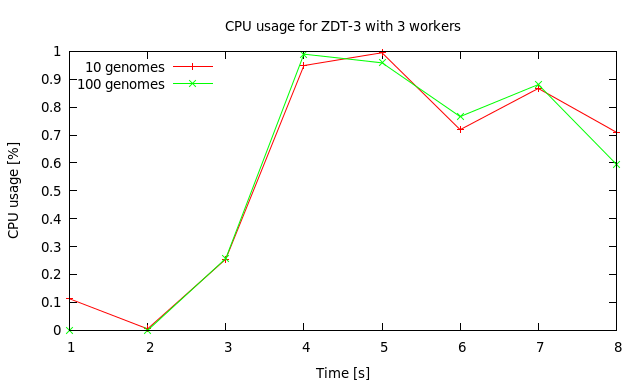
\includegraphics[width=90mm,natwidth=640,natheight=384]{cpu_10_100.png}
  \caption[CPU usage for ZDT-3, 10 and 100 genomes, 3 workers]{CPU usage for ZDT-3, 10 and 100 genomes, 3 workers - 250 iterations}
  \label{fig:cpu_10_100}
\end{figure}

It is arguable that the AET of ZDT-3 with 10 and 100 genomes is to short to get correct informations about the CPU usage. Therefore, the ZDT-3 benchmarks for 3 workers with 10 and 100 genomes were performed for 1000 iterations (original benchmarks iterate only 250 times). The results can be seen in fig. \ref{fig:cpu_10_100-1000-iter}. They confirm the CPU saturation for ZDT-3 with 10 and 100 genomes and three and more workers.

\begin{figure}
  \centering
  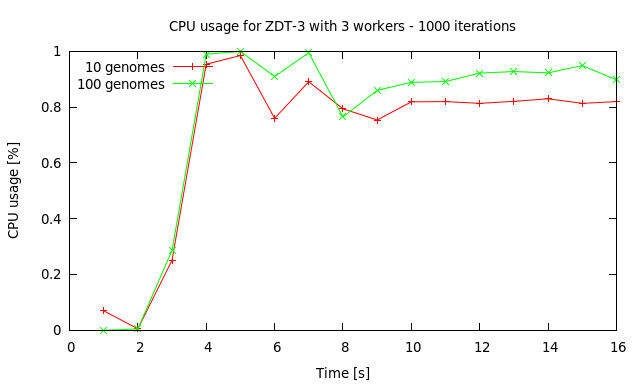
\includegraphics[width=90mm,natwidth=640,natheight=384]{cpu_10_100-1000-iter.png}
  \caption[CPU usage for ZDT-3, 10 and 100 genomes, 3 workers]{CPU usage for ZDT-3, 10 and 100 genomes, 3 workers - 1000 iterations}
  \label{fig:cpu_10_100-1000-iter}
\end{figure}

Since the master executes the sequential parts of the algorithms and in addition has to communicate with all workers, it is clear that a saturation of the master CPU prevents further performance gains. The problem worsens when additional YARN containers run on the computer that executes the master.

% The high CPU utilization is caused by two effects. The first one is the object serialization/deserialization and communication overhead performed on the master that ranges from about \unit[30]{\%} to \unit[50]{\%} for genome sizes of 10 and 100. This numbers were established by profiling Biohadoops master with the honest-profiler\footnote{\url{https://github.com/RichardWarburton/honest-profiler} last access: 27.01.2015}. The profile results were used to generate a flame graph 
% 
% goes up to \unit[60]{\%} to \unit[70]{\%} for a genome size of 10000. Small genome sizes mean a high rate of both exchanged messages and serializations/deserializations. Large genome sizes reduce the rate of exchanged messages but increase the amount of work for a single serialization/deserialization.
% 
% The second effect is a direct consequence of computationally small worker tasks like in the case of 10 to 100 genomes: the master performs (beside the communication aspects) the algorithms for ranking and crowding distance. The workers return their results fast as the computation is not intense. Therefore, the master has to compute the ranking and crowding distance at short intervals. This results in a CPU utilization of about \unit[25]{\%} to \unit[30]{\%} only for this computations.
% 
% TMMs behave very differently. The workers execute compute intense matrix multiplications, communication between the master and its workers occurs seldom. In addition, the amount of data sent between the master and the workers consists only of tile sizes for $i$, $j$ and $k$ (see TMM description in section \ref{chap:evaluation:tiledmul}). The result is an execution pattern that poses high CPU loads onto the worker, the master CPU instead is has less work to do. Message are exchanged on a rarely basis and the size of exchanged messages is small.
% 
% In conclusion, the ZDT-3 benchmarks are CPU bound by the master due to the small computational effort on the workers and the resulting fast exchange of many small messages. Increased genome sizes provide better speedup results, but are again limited by the CPU of the master, as they have higher demands for object serialization/deserialization. TMM in contrast has more favorable properties: compute intense fitness evaluations on the workers and small message sizes. Those properties result in significantly decreased AETs and better parallel performance.

\subsection{Other influences}
\label{chap:evaluation:influence-other}
YARN and the CPU had the biggest effects on the benchmark results. In the following, other possible influencing factors are summarized. Their impact on the benchmark results is not quantified, as their correct evaluation is not trivial but very work intensive. As already mentioned, further research projects could develop tools to simplify this process.

\begin{description}
  \item [Network]: The network influences the benchmark results, as the master and its workers exchange messages through it. This influence is apparent in cases where YARN places its containers on the same computer, which can result in greatly reduced AETs. Nevertheless, the network influence is consistent: throughput and latency don't change over the time on the used test cluster.
  \item [RAM]: All benchmarks start with \unit[256]{MB} of Java heap memory which is enough for the containers to execute without causing excessive garbage collections. This was established by using the tool jvisualvm\footnote{\url{http://visualvm.java.net/} last access: 26.01.2015} (delivered with Java) for the ZDT-3 benchmark with 10000 genomes and the TMM with a matrix size of 256$\times$256. The memory usage for the master container is at about \unit[100]{MB} to \unit[150]{MB}. The memory usage for a worker is even lower and lies in the range of \unit[5]{MB} to \unit[30]{MB}. The conclusion is, that enough RAM was available during the benchmarks. To few RAM would have had significant impact on the performance.
  \item [CPU caches]: The CPU caches show their biggest influence during the TMM benchmarks. The workers execute matrix multiplications using provided tile sizes. If the tiles are small enough they fit into the L1 CPU cache which is the fastest memory available to a processor. Increased performance is the result. If the tiles don't fit into L1 cache, they need to be retrieved from L2 cache or even worse from main memory, which introduces latencies. Since TMM executes matrix multiplications to evaluate the fitness of an individual, the tile sizes affect the fitness evaluation of a single individual, and the whole runtime of the benchmark.
  \item [Java Java Just in Time Compiler (JIT)]: JIT\footnote{\url{http://en.wikipedia.org/wiki/Just-in-time_compilation} last access: 26.01.2015} compiles Java byte code into machine executable code that can be executed faster. During the benchmarks, JIT was set to optimize code parts that are executed more than 10000 times (this is the standard setting for the used Java Server runtime\footnote{\url{http://en.wikipedia.org/wiki/HotSpot} last access: 26.01.2015}). Small benchmarks, like ZDT-3 with 10 genomes, hit this threshold later in their execution. Therefore, the share of executed un-optimized code is larger compared to large benchmarks, e.g., ZDT-3 with 10000 genomes. This problem worsens with increasing numbers of workers.
  \item [Operating system (OS)]: The OS provides the basis for application execution. It provides also the interfaces for hardware usage, e.g. network communication. Therefore, it has large influence on executed applications. Using the right drivers and OS settings, e.g., for buffers, influence the performance of running applications significantly.
  \item [Building blocks]: Biohadoop uses Netty and Kryo for the communication between the master and its workers. Those libraries can be configured in many different ways. Again, the right configuration can provide performance increases or degradations.
\end{description}

\section{Speedup}
\label{chap:evaluation:speedup}
Speedup is a metric that tells how many times a parallel version of an algorithm (or system) runs faster compared to the sequential version. In the following, the maximum achievable speedups and the experimental speedup, i.e., the speedup achieved in the benchmarks, are presented in section \ref{chap:evaluation:max_speedup} and \ref{chap:evaluation:exp_speedup}, respectively.

\subsection{Maximum achievable Speedup}
\label{chap:evaluation:max_speedup}
The max. achievable speedup ($S_{max}$) for a given problem is the best-case result achievable through parallelization. It is computed using Amdahl's law \cite{amdahl1967validity}:

\begin{equation}
S_{max} = T / (T - t_p)
\end{equation}

In this formula, $T$ is the sequential execution time of an algorithm. During this sequential execution it is also measured how much time is spent in code parts that could be executed in parallel. This amount of time is defined as $t_p$.

The values for $T$ and $t_p$ are taken from the benchmark executions with a single worker. Since the measured AET for a given benchmark and one worker differs largely (e.g. ZDT-3 with 100 genomes), lower and upper max. achievable speedup boundaries are computed. The lower bound is computed using the worst sequential-to-parallel execution time ratio of a sequential benchmark run. The upper bound reflects the best sequential-to-parallel ratio. This proceeding gives more details over the achievable speedups.

Table \ref{table:achievable_speedups} presents the lower and upper bounds for the max. achievable speedups based on the benchmark results. The calculations show that ZDT-3 is generally not well suited for parallelization. In the best case with 1000 workers its performance can be increased by a factor of about 20 (upper bound). In the worst case with 10 genomes the performance can be increased by a factor of 5 (lower bound). The reason for the small achievable speedups is the bad sequential-to-parallel execution time ratio. ZDT-3 as fitness function is barely compute intense. As the fitness function is usually (but not in this case) the most compute intense part of an optimization, this leads to the mentioned bad sequential-to-parallel execution time ratio.

\begin{table}
  \centering
  \caption{Lower and upper bounds for max. achievable speedups}
  \begin{tabular}{lrrrr}\toprule[2pt]
    Test Problem & \parbox[r]{3.5cm}{Lower Achievable Speedup Boundary}& \parbox[r]{3.5cm}{Upper Achievable Speedup Boundary}\\ \midrule
    NSGA-II, 10 genomes & 4.816 & 11.046 \\
    NSGA-II, 100 genomes & 5.228 & 9.398 \\
    NSGA-II, 1000 genomes & 9.438 & 20.275 \\
    NSGA-II, 10000 genomes & 8.861 & 17.081 \\
    TMM, 128$\times$128 & 63.649 & 134.404 \\
    TMM, 256$\times$256 & 139.685 & 271.925 \\ \bottomrule[2pt]
  \end{tabular}
  \label{table:achievable_speedups}
\end{table}

TMM on the other side shows better results. It demonstrates that the test problem is well suited for parallelization. This is not surprising, as the parallel part in form of the fitness evaluation consists of a matrix multiplication which is known to be compute intensive. Therefore, the sequential-to-parallel execution time ratio is advantageous and opens the possibility to achieve good experimental speedups.

\subsection{Experimental Speedup}
\label{chap:evaluation:exp_speedup}
To compute the experimental speedup $S$ for a given benchmark, its sequential ($T_S$) and parallel ($T_P$) execution times are needed. $T_S$ is the execution time for a benchmark with a single worker. $T_P$ is the execution time for a benchmark with $P$ workers. $S$ is then calculated using the following formula:

\begin{equation}
S = T_S / T_P
\end{equation}

Since the execution times for a given benchmark and setting vary often in a broad range, the lower and upper speedup boundaries for a given benchmark are computed. This is the same proceeding used for the computation of the max. achievable speedups. The boundaries are computed by using the min. and max. execution times for $T_S$ and $T_P$, respectively. For example, min. $T_S$ and max. $T_P$ of a given benchmark and setting are used to compute the lower speedup boundary. Max. $T_S$ and min. $T_P$ are used to compute the upper speedup boundary.

Fig. \ref{fig:speedup_min} shows the lower speedup bounds for all benchmarks, fig. \ref{fig:speedup_max} the upper speedup bounds. The figures demonstrate that the speedups for ZDT-3 benchmarks are small. Even when looking at the best case of upper bound speedups it is clear that ZDT-3 takes little profit of the parallelization. The lower bounds of the experimental speedups show even poorer results. This comes at no surprise, since the max. achievable speedups computed in section \ref{chap:evaluation:max_speedup} are already small and it is very unlikely to reach them in practice.

\begin{figure}
  \centering
  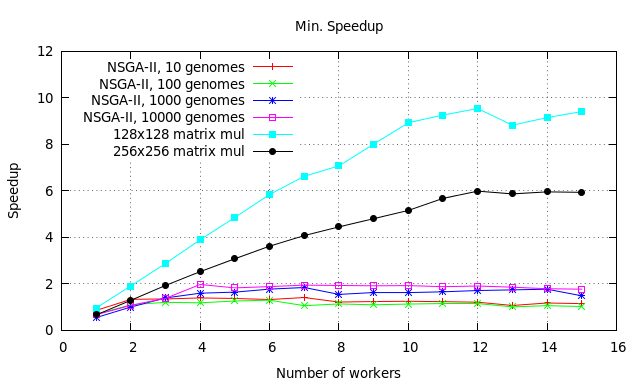
\includegraphics[width=100mm,natwidth=640,natheight=384]{speedup_min.png}
  \caption[Min. speedups for ZDT-3 and TMM benchmarks]{Lower speedup boundaries for ZDT-3 and TMM benchmarks}
  \label{fig:speedup_min}
\end{figure}
\begin{figure}
  \centering
  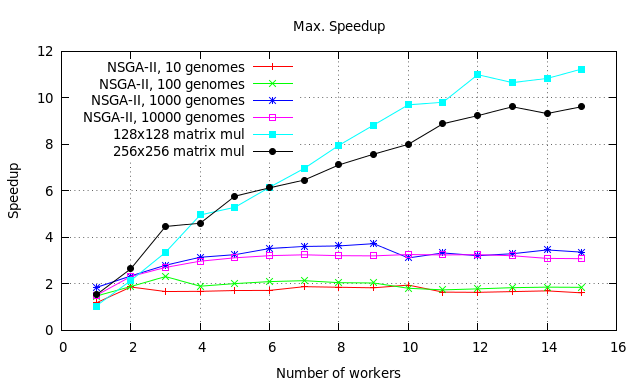
\includegraphics[width=100mm,natwidth=640,natheight=384]{speedup_max.png}
  \caption[Max. speedups for ZDT-3 and TMM benchmarks]{Upper speedup boundaries for ZDT-3 and TMM benchmarks}
  \label{fig:speedup_max}
\end{figure}

In contrast, the TMM results show good speedup behaviours. The benchmarks with a matrix size of 128$\times$128 demonstrate almost linear performance increases, which tend to be super-linear for the upper bound speedups. Super-linear speedups are usually suspicious. In this case they can be explained by the way the boundaries of the experimental speedups are computed. Nevertheless, also the lower bounds for TMM benchmarks with a matrix size of 128$\times$128 show almost linear increases. All speedups of all TMM benchmarks reach their maximum when 10 to 12 workers are used. This observation matches with the fact, that the whole cluster provides 12 cores.

The reason for the worse speedup of 256$\times$256 TMM compared to the 128$\times$128 version lies in the bigger solution space of 256$\times$256 TMM. It is more likely to find bad performing tile sizes for bigger matrices. The L1 cache sizes are limited and to big tile sizes affect the performance negatively.

The conclusion of the speedup results is that the parallelized search for values that minimize the ZDT-3 function is not well suited for Biohadoop --- at least for the used implementation. More advanced implementations may influence the sequential-to-parallel ratio and achieve better results. A different, more compute intense fitness function may also entail better speedup results. TMM on the other side provides good speedups and decrease the AET by a large amount. The parallelized search for optimal tile sizes using Biohadoop is favorable.


% \subsection{Network Influence}
% This section examines if the benchmarks hit the data transfer limit of the used \unit[1]{Gb} Ethernet. This would have a big impact on their execution times. Please note that from here on the data units are distinguished as follows: a small ``b'' denotes bits, a big ``B'' denotes bytes, e.g., \unit[1]{Gb} = 1 gigabit, \unit[1]{GB} = 1 gigabyte.
% 
% All benchmarks perform 250 iterations on 100 individuals, resulting in 25000 tasks. The tasks are send from the master to the workers and the workers return the results. The task data send from the master to the worker contains two individuals.
% 
% For ZDT-3, each individual consists of its genome, where each value in the genome is of type \texttt{double} (8 bytes). For a genome size of 10, this makes 2 (parents) $\times$ 10 (genomes) $\times$ 8 (bytes) $\times$ 25000 (tasks) = 4000000 bytes (\unit[4]{MB}) or \unit[32]{Mb} of data that needs to be transferred from the master to the workers during the benchmark.
% 
% The amount of transmitted data for TMM is far less, since each genome constantly consists of three tile size $i$, $j$ and $k$. Each tile size is of type \texttt{integer} (4 bytes). This gives a total of 2 (parents) $\times$ 3 (genomes) $\times$ 4 (bytes) $\times$ 25000 (tasks) = 600000 bytes or \unit[4.8]{Mb} of data.
% 
% Table \ref{table:network} sums the amounts of data that need to be transferred and gives a theoretical transfer time for the \unit[1]{Gb} Ethernet used in the cluster. It provides also information about the fastest execution time of a given benchmark. The results show that for the given benchmarks the data can be moved between the master and the workers without hitting the network transfer limit.
% 
% \begin{table}
%   \centering
%   \begin{tabular}{r|r|r|r}
%     Benchmark & data [Mb] & \parbox[t]{3cm}{theoretical\\transfer time [s]} & \parbox[t]{3cm}{fastest algorithm\\execution time [s]}\\ \hline
%     NSGA-II, 10 genomes & 32 & 0.032 & 7.072 \\
%     NSGA-II, 100 genomes & 320 & 0.32 & 7.031 \\
%     NSGA-II, 1000 genomes & 3200 & 3.2 & 8.910 \\
%     NSGA-II, 10000 genomes & 32000 & 32 & 55.475 \\
%     TMM, 128x128 & 4.8 & 0.0048 & 18.386 \\
%     TMM, 256x256 & 4.8 & 0.0048 & 178.158 \\
%   \end{tabular}
%   \caption{Amount of network data sent from master to workers, theoretical transfer time and fastest algorithm execution}
%   \label{table:network}
% \end{table}
% 
% Additional experiments were performed to improve the confidence in the calculations and to establish the true achievable data rate for the network, given different message sizes. The experiments measure the peak network bandwidth using a small Java program and iftop.\footnote{\url{http://www.ex-parrot.com/pdw/iftop/} last access: 08.12.2014} The Java program uses the same communication techniques as Biohadoop (Netty + Kryo) and performs repeated request/response cycles between a master and several workers. The achieved data rates were \unit[134]{Mb/s} for 20 \texttt{doubles} and \unit[489]{Mb/s} for 200 \texttt{doubles}, according to ZDT-3 genome sizes of 10 and 100. Using 2000 \texttt{doubles}, the transfer data rate peaked at \unit[901]{Mb/s} which is near to the theoretical limit of the network. For 20000 \texttt{doubles} the data rates dropped again to \unit[552]{Mb/s}, in addition the CPU utilization was reduced notably to about \unit[40]{\%}. The reason for this behaviour could not be established. A possible explanation is that necessary data copies consumed a lot of time in the underlying operating system (Linux with kernel 3.13), Kryo, Netty or the Java runtime in general.
% 
% Further research projects could provide support tools to get detailed network performance data in Hadoop environment. This would be beneficial since it is a difficult process to gain the network data. For example, YARN containers can be executed on every available computer of a cluster. One has to determine first where the containers are located before the network performance can be measured.
% 

\section{Comparison to Standalone Implementations}
\label{chap:evaluation:comparison}
Standalone, sequential benchmarks ($SB$) of the test problems in section \ref{chap:evaluation:testproblems} are executed to determine if the algorithm parallelization using Biohadoop is advantageous. $SB$ are written in Java and executed on a single cluster machine. They use the same algorithm implementations and settings as the parallel versions, but run without Biohadoop and its task system. This entails that they perform no network communication at all.

Table \ref{table:sequential-runtimes} shows the fastest standalone sequential execution times ($T_S$), together with the fastest execution times achieved with parallel implementations ($T_P$). It provides also information about the speedup gained through parallelization. This speedup is computed the same way as in section \ref{chap:evaluation:exp_speedup}. The speedup is abbreviated with letter $G$ (gain) for better distinction to the previous results:

\begin{equation}
G = T_S / T_P 
\end{equation}

If $G$ is smaller than 1, the parallelization has a negative effect and should be avoided. In this cases, the parallel execution takes longer than the sequential execution. Values for $G$ that are bigger than 1 are favorable, since they provide reduced execution times.

\begin{table}
  \centering
  \caption[Execution times for standalone sequential implementations]{Execution times for $SB$}
  \begin{tabular}{lrrr}\toprule[2pt]
    Test Problem &  Sequential [s] & Parallel [s] & Performance gain \\ \midrule
    NSGA-II, 10 genomes & 2.852 & 6.461 & 0.441 \\
    NSGA-II, 100 genomes & 2.956 & 6.128 & 0.482 \\
    NSGA-II, 1000 genomes & 7.673 & 8.330 & 0.921 \\
    NSGA-II, 10000 genomes & 71.390 & 53.706 & 1.329 \\
    TMM, 128$\times$128 & 132.066 & 18.386 & 7.183 \\
    TMM, 256$\times$256 & 1500.705 & 178.158 & 8.423 \\ \bottomrule[2pt]
  \end{tabular}
  \label{table:sequential-runtimes}
\end{table}

The ZDT-3 benchmarks for genome sizes up to 1000 show that the parallelization has a negative impact, the parallel execution times are bigger than the serial execution times. In this cases, it is better to stick with the serial implementation. ZDT-3 with a genome size of 10000 shows that the execution of parallel versions provide advantages in terms of execution time, although the performance gains are not very big.

The situation is completely different for the TMM benchmarks. The parallel implementations provide large benefits compared to the sequential versions.


% \section{Sequential Benchmarks}
% \label{chap:evaluation:sequential}
% Sequential benchmarks ($SB$) of the test problems in section \ref{chap:evaluation:testproblems} are executed to get basis execution time results. The results are used to compute the max. speedups that are achievable through parallelization. The second purpose of $SB$ is execution time comparison to the parallel versions in section \ref{} to determine if the parallelization is advantageous.
% 
% $SB$ are written in Java and executed on a single cluster machine. They use the same algorithm implementations and settings as the parallel versions, but run without Biohadoop and its task system. This entails that they perform no network communication at all.
% 
% % Each $SB$ is repeated five times. The best and worst sequential-to-parallel execution time ratios for each benchmark type are used to compute the speedup boundaries of the parallel Biohadoop versions.
% 
% \subsection{Sequential Execution Times and Achievable Speedups}
% \label{chap:evaluation:sequential-exec-time}
% $SB$ are used to establish the max. achievable speedups for the parallel benchmarks ($PB$). This is accomplished by measuring the $SB$ execution time ($T$) and the time spent in its parallelizable code parts ($t_p$). $T$ is simply the time the Java program takes to complete. The max. achievable speedup $S$ is then computed using Amdahl's law \cite{amdahl1967validity}:
% 
% \begin{equation}
% S = T / (T - t_p)
% \end{equation}
% 
% Since each $SB$ is repeated five times, average values for the execution times and the time spent in parallel code parts are used for the achievable speedup computations. Table \ref{table:achievable_speedups} shows the results for $T$, $t_p$ and the achievable speedups.
% 
% \begin{table}
%   \centering
%   \caption{$SB$ benchmark results and max. achievable speedups}
%   \begin{tabular}{lrrrr}\toprule[2pt]
%     Test Problem & $T$ [s] & $t_p$ [s] & Achievable Speedup \\ \midrule
%     NSGA-II, 10 genomes & 14.535 & 13.339 & 12.153 \\
%     NSGA-II, 100 genomes & 15.232 & 13.530 & 8.949 \\
%     NSGA-II, 1000 genomes & 42.485 & 38.718 & 11.278 \\
%     NSGA-II, 10000 genomes & 358.961 & 327.968 & 11.582 \\
%     TMM, 128$\times$128 & 769.840 & 766.116 & 206.724 \\
%     TMM, 256$\times$256 & 7743.585 & 7714.341 & 264.792 \\ \bottomrule[2pt]
%   \end{tabular}
%   \label{table:achievable_speedups}
% \end{table}
% 
% ZDT-3 benchmarks have the smallest achievable speedups. This gives a hint that their parallelization will not have much impact on the execution times, e.g., NSGA-II with 10 genomes can reduce its execution time by a factor of 12.153 at most --- no matter how much computational resources are involved. The poor results are the consequence of the short amount of time spent in parallelizable code parts, compared to the sequential part. The parallel code parts involve offspring creation and fitness evaluation using the ZDT-3 function (see section \ref{chap:evaluation:zdt3}). Fitness evaluation is usually a compute intense task, but for the ZDT-3 function this is not the case. This leads to a bad sequential-to-parallel ratio and hence to the bad achievable speedups.
% 
% The TMM benchmarks promise better results with max. achievable speedups of over 200. The parallelizable code parts of TMM are, like for ZDT-3, offspring creation and fitness evaluation. In the case of TMM the fitness evaluation involves a compute intense matrix multiplication. This leads to a good sequential-to-parallel ratio and provides the possibility for high speedups.


% \section{Parallel Benchmarks using Biohadoop}
% \label{chap:evaluation:parallel}
% The $AET$ results for the parallel benchmarks are presented in fig. \ref{fig:nsga_250_100_10} to \ref{fig:nsga_250_100_10000} for the ZDT-3 test problem. Fig. \ref{fig:tiledmul_250_100_128x128} and \ref{fig:tiledmul_250_100_256x256} show the results for the TMM benchmarks.

% Its not easy to give and interpretation of the results. Especially 

% The NSGA-II results for genome sizes of 10 and 100 have the interesting property that the $AET$ for a given setting typically varies over a broad range.
% 
% The NSGA-II results have the interesting property that the $AET$ for a given benchmark and setting (e.g. NSGA-II, 10 genomes) typically varies over a broad range. This is unexpected since each benchmark is repeated five times and the repetitions should provide comparable results. This leads to the conclusion that the executions are influenced by different factors.

% An interesting thing to note when looking at the results is that $AET$ for a given setting (e.g. NSGA-II, 10 genomes) and one worker differ by a large amount. The explanation for this effect is the behaviour of YARN.

% One can see that the ZDT-3 $AET$ reduce only by a small amount when the number of workers is increased. The biggest performance gain is This results coincide with the achievable speedup computations of section \ref{chap:evaluation:sequential-exec-time}. Nevertheless, they are worse than expected. TMM on the other side performs very well and profits from the parallelization.

% \subsection{Network Influence}
% The ZDT-3 benchmarks seem to suffer from the lack of one or more resources (bound by the resources), which prohibits further speedup increases. The investigations show that the ZDT-3 benchmarks are not bound by memory, i.e., memory issues don't slow the execution down. All benchmarks start with \unit[256]{MB} of Java heap memory, which is enough for the containers to execute without causing excessive garbage collections. This was established by using the tool jvisualvm (delivered with Java) for the ZDT-3 benchmark with 10000 genomes. The memory usage for the master container is at about \unit[100]{MB} to \unit[150]{MB}. The activity of Java's garbage collector, a good indicator for memory problems, ranges from \unit[3]{\%} to \unit[5.5]{\%} of the CPU time, with an average of \unit[3.8]{\%}. The memory usage for a worker is even lower and lies in the range of \unit[5]{MB} to \unit[30]{MB}. This numbers show no significant memory problems.
% 
% The next step is to investigate the network performance. Calculations give a first hint to understand if the bad speedups can be explained with the saturation of the \unit[1]{Gb} network (a small ``b'' denotes bits, a big ``B'' denotes bytes, e.g., \unit[1]{Gb} = 1 gigabit, \unit[1]{GB} = 1 gigabyte). In each benchmark, 250 iterations on 100 individuals are performed, resulting in 25000 tasks. The tasks are send from the master to the workers and the workers return the results. The task data send from the master to the worker contains two individuals. Each individual consists of its genome, where each value in the genome is of type \texttt{double} (8 bytes). For a genome size of 10, this makes 2 (parents) $\times$ 10 (genomes) $\times$ 8 (bytes) $\times$ 25000 (tasks) = 4000000 bytes (\unit[4]{MB}) or \unit[32]{Mb} of data that needs to be transferred from the master to the workers during the benchmark. The size of the results sent from the workers to the master is about the half, as it consists of an individual (the offspring) and its fitness (the fitness is composed of two \texttt{double} values). This fact allows to use the outgoing data amount as upper bound for the network usage: if the outgoing data rate doesn't exceed the network bandwidth. This will be true also for the incoming data. Table \ref{table:network} shows the results for all genome sizes together with the best algorithm execution times. One can see from the table that the benchmark data can be transferred on the \unit[1]{Gb} Ethernet network during the according fastest algorithm execution time.
% 
% \begin{table}
%   \centering
%   \begin{tabular}{r|r|r|r}
%     genomes & data [Mb] & \parbox[t]{3cm}{theoretical\\transfer time [s]} & \parbox[t]{3cm}{fastest algorithm\\execution time [s]}\\ \hline
%     10 & 32 & 0.032 & 7.072 \\
%     100 & 320 & 0.32 & 7.031 \\
%     1000 & 3200 & 3.2 & 8.910 \\
%     10000 & 32000 & 32 & 55.475 \\
%   \end{tabular}
%   \caption{Amount of network data sent from master to workers, theoretical transfer time and fastest algorithm execution}
%   \label{table:network}
% \end{table}
% 
% Additional experiments were performed to improve the confidence in the calculations and to establish the true achievable data rate for the network, given different message sizes. The experiments measure the peak network bandwidth using a small Java program and iftop.\footnote{\url{http://www.ex-parrot.com/pdw/iftop/} last access: 08.12.2014} The Java program uses the same communication techniques as Biohadoop (Netty + Kryo) and performs repeated request/response cycles between a master and several workers. The exchanged messages consist of 20, 200, 2000 or 20000 \texttt{double} values, corresponding to two parent individuals in the according ZDT-3 benchmarks. The resulting peak bandwidth was \unit[134]{Mb/s} for 20, \unit[489]{Mb/s} for 200, \unit[901]{Mb/s} for 2000 and \unit[552]{Mb/s} for 20000 \texttt{double} values. The CPU on the master was the limiting factor for 20, 200 and 20000 \texttt{double} values. For 2000 \texttt{double} values, the network was saturated at \unit[901]{Mb/s} and, therefore, the limiting factor. No studies were performed to explain why the experiments delivered the best results with 2000 values as this lies out of the scope of this thesis.
% 
% One phenomena regarding the network bandwidth needs further investigation. The above measurements show a peak data rate of \unit[552]{Mb/s} for the case of 20000 \texttt{double} values. If this data rate is taken as a basis for the ZDT-3 benchmark with 10000 genomes, one can calculate that more than \unit[55]{s} are needed to exchange \unit[32]{Gb} of data over the network between the master and its workers (\unit[32000]{Mb} / \unit[552]{Mb/s} = \unit[57.97]{s}). The explanation can be found once more in the YARN container placement. The \unit[552]{Mb/s} peak bandwidth is the data rate that is send through the Ethernet port to the cluster, but worker containers that run on the same machine as the master don't use this port for communication. Instead, they communicate through the local interface. iftop showed an additional combined data transfer rate of \unit[400]{Mb/s} (send and receive data rates are added) on the local interface when workers were running on the same machine as the master. This gives an aggregated peak data rate of \unit[700]{Mb/s} to \unit[800]{Mb/s} for the outgoing traffic, which is fast enough to transmit \unit[32]{Gb} of data in less than \unit[55]{s}. The execution times were higher in cases where no workers executed on the same machine as the master.
% 
% The calculations and additional experiments show that the network is fast enough to transfer the ZDT-3 benchmark data. The reason for the bad ZDT-3 speedups lie elsewhere.
% 
% \subsection{RAM Influence}
% All benchmarks start with \unit[256]{MB} of Java heap memory, which is enough for the containers to execute without causing excessive garbage collections. This was established by using the tool jvisualvm (delivered with Java) for the ZDT-3 benchmark with 10000 genomes and the TMM with a matrix size of 256x256. The memory usage for the master container is at about \unit[100]{MB} to \unit[150]{MB}. The activity of Java's garbage collector at the master takes about \unit[5]{\%} of the CPU time. This value would be significantly higher in case of a memory problem. The memory usage for a worker is even lower and lies in the range of \unit[5]{MB} to \unit[30]{MB}. Again, this numbers show no significant memory problems.
% 
% \subsection{CPU Influence}
% 
% \subsection{Cache Influence}
% 
% \subsection{Network Influence}
% 
% \section{Speedup}
% \label{chap:evaluation:speedup}
% The speedup properties of Biohadoop are established using the test problems mentioned in section \ref{chap:evaluation:testproblems}. They were chosen because they implement well known bio-inspired optimization techniques (GA and NSGA-II) used in real world scenarios, e.g. bridge construction (!!!! JUANJO!!!!).
% 
% The following formula was used to compute the speedup:
% 
% \begin{equation}
% S = T_S / T_P
% \end{equation}
% 
% Here, $S$ is the speedup. The sequential time $T_S$ is taken from the execution time of the test problems with a single worker. $T_P$ is the time for the execution with 2 to 15 parallel workers.
% 
% Different factors influence the execution times on Hadoop, e.g. CPU, network, YARN. At this point it is only important to know that such factors exist (more information about them can be found in section \ref{chap:evaluation:discussion}). Because of the large influence of the factors on the algorithm execution times, the speedup computations are performed based on min. and max measurements for each benchmark setting. This provides speedup boundaries that give more information about the speedup characteristics compared to average values.
% 
% 
% 
% \subsection{Speedup Results}






% The start up time over all benchmarks range from \unit[2.378]{s} to \unit[6.147]{s}, with a median of \unit[3.864]{s}, a \unit[25]{\%} quartile of \unit[3.145]{s} and a \unit[75]{\%} quartile of \unit[4.258]{s}. The mean value is \unit[3.781]{s}. These start up times are close to each other, because the used cluster was completely dedicated to the benchmarks. The start up may take longer when the cluster usage is higher.

% The algorithm execution time results for the benchmarks can be found in the boxplots in figures \ref{fig:nsga_250_100_10} to \ref{fig:nsga_250_100_10000} for the ZDT-3 benchmarks and in figures \ref{fig:tiledmul_250_100_128x128} and \ref{fig:tiledmul_250_100_256x256} for the TMM. The number of workers and the algorithm execution time is plotted on the x-axis and y-axis, respectively.

% \subsection{Parallel Benchmarks using Biohadoop}
% The execution times of $SB$ and $PB$ are needed to compute the true speedups and therefore evaluate if it is feasible to use Biohadoop for parallelization. In the prior chapter speedup boundaries were established to have a better overview of the achieved results. This concept is applied also to the $PB$ benchmarks. But first, some definitions have to be made.
% 
% \subsubsection{Parallel speedups}
% The algorithm execution times using the Biohadoop version of the benchmarks are measured and used to calculate the speedups for the benchmarks using the formula $S = T_S / T_P$. Here, $S$ is the speedup. The sequential time $T_S$ is taken from $SB$. $T_P$ is the time for the execution with 1 to 15 parallel workers.
% 
% Figure \ref{fig:speedup} depicts the speedups for all test problems with respect to increasing worker sizes. The ZDT-3 benchmarks show poor results. This is not surprising as the maximum theoretical speedups of this problem are small (see table \ref{table:speedup_bounds}) and the communication overhead is bigger compared to TMM. The only unexpected outcome was that the benchmarks scale very bad with a maximum speedup of 2.498 for 1000 genomes. The reason is that the ZDT-3 benchmarks are CPU bound by the master, as the investigations in section \ref{chap:evaluation:result:zdt3} suggest.
% 
% TMM demonstrate better results, the maximum speedup was 10.507 for a matrix size of 128$\times$128. In this case, the speedup grows near linear or even slightly better than linear with the number of workers. That a speedup is better than linear is usually suspicious but can be explained by the fact that each benchmark was repeated five times and the average times of this five executions were taken to compute the speedups. Five executions seem to be too small for getting smooth results, especially when taking into account that the YARN container placement has big influences on the execution times.
% 
% The speedups for the 128$\times$128 TMM increase until a worker size of 12 is reached. At this point, no more improvements are achieved. The reason for this is the limited number of CPUs in the cluster.
% 
% The speedup for the 256$\times$256 TMM benchmark is worse compared to the 128$\times$128 TMM, although it also grows nearly linear until 12 workers.
% 
% \begin{figure}
%   \centering
%   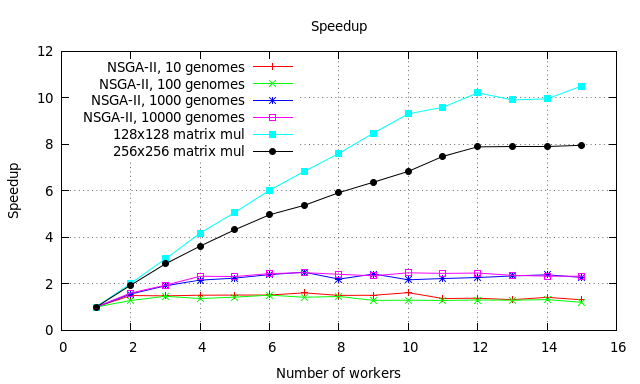
\includegraphics[width=130mm,natwidth=640,natheight=384]{speedup.png}
%   \caption[Speedups for ZDT-3 and TMMs]{Speedups for ZDT-3 and TMMs}
%   \label{fig:speedup}
% \end{figure}
% 
% \subsection{Speedup Comparison}
% 
% \subsection{Feasibility of Results}



% \begin{itemize}
%   \item Free resources (CPU, RAM, Network) on the machine: The utilization of a machine by other processes influences the execution times.
%   \item Network package size: The network in use has a maximum package size. If data packets exceed this size, they need to be chunked into several smaller packets.
%   \item JIT (Just-in-time compiler): the Java just-in-time compiler compiles Java byte code into machine executable code that can be executed faster. This compilation is done only if a a certain part of a Java program is called several times (typically after 10000 calls). JIT optimized code executes faster than interpreted code, but takes itself some time to get compiled
%   \item Netty and Kryo performance: Netty provides the network functionality for Biohadoop, Kryo is used for serialization. Both are executed on the master and worker processes and have influence on the algorithm execution times due their need for resources. It is hard to estimate how Netty and Kryo behave for different data sizes, e.g., kt is tunable how much buffer memory Kryo allocates by default for serialization/deserialization. 
%   \item L1 / L2 cache sharing and pollution: The CPUs used for the benchmarks have a per-core L1 cache of \unit[32]{KB} and a shared L2 cache of \unit[6]{MB}. Since several processes run on each machine (.e.g. the operating system and the Hadoop processes), it is hard to estimate how much cache is available for the benchmark execution.
%   \item YARN container placement: The benchmark algorithm execution times depend on the placement of the YARN containers.
%   \item YARN container startup time (master and worker containers): It may take arbitrary time for YARN to start a container. This can not be influenced.
%   \item Operating System (OS): The OS needs resources itself. It provides the resources for the benchmark execution and the transmission of network data. Especially the second component can have an influence on the execution times.
% \end{itemize}

% Table \ref{table:theoretical_speedup} gives an impression how well the benchmark problems are suited to parallelization by showing the maximum theoretical speedup. The theoretical speedup was calculated using the formula $S = T / (T - t_p)$ from Amdahl's law \cite{amdahl1967validity}, where $S$ is the speedup, $T$ the algorithm execution time and $t_p$ is the time spent in code parts that are parallelized using Biohadoops task system. $T$ and $t_p$ were taken from the average benchmark times with one worker.

% \begin{table}
%   \centering
%   \caption{Theoretical speedups}
%   \begin{tabular}{lr}\toprule[2pt]
%     Test Problem & Theoretical Speedup \\ \midrule
%     NSGA-II, 10 genomes & 7.028 \\
%     NSGA-II, 100 genomes & 7.600 \\
%     NSGA-II, 1000 genomes & 12.008 \\
%     NSGA-II, 10000 genomes & 11.124 \\
%     128$\times$128 tiled mul & 81.359 \\
%     256$\times$256 tiled mul & 212.169 \\ \bottomrule[2pt]
%   \end{tabular}
%   \label{table:theoretical_speedup}
% \end{table}

% One can see from the theoretical speedups that ZDT-3 is not well suited for parallelization. This is due to the fact that the fitness evaluation is not compute intense. Its time consuming part is a sum over the genomes of an individual, implemented as loop. For example, in the case of 10 genomes per individual this loop would be repeated 10 times. Bigger genome sizes mitigate this effect but have the drawback that the communication time between the master and the workers increases, which negatively affects the speedup. TMMs on the other side show a big potential for parallelization.

% \subsection{ZDT-3}
% \label{chap:evaluation:result:zdt3}
% The next thing to notice are the speedups for the ZDT-3 benchmarks. ZDT-3 is not well suited for parallelization as can be seen from the speedups in table \ref{table:speedup_bounds}, but the results are even worse than expected, with maximum speedups of 1.619 for 10 genomes, 1.513 for 100 genomes, 2.498 for 1000 and 2.479 for 10000 genomes. Figure \ref{fig:speedup} shows the speedup results of the ZDT-3 benchmarks together with the speedups for TMM.
% 
% 
% 
% The ZDT-3 benchmarks seem to suffer from the lack of one or more resources (bound by the resources), which prohibits further speedup increases. The investigations show that the ZDT-3 benchmarks are not bound by memory, i.e., memory issues don't slow the execution down. All benchmarks start with \unit[256]{MB} of Java heap memory, which is enough for the containers to execute without causing excessive garbage collections. This was established by using the tool jvisualvm (delivered with Java) for the ZDT-3 benchmark with 10000 genomes. The memory usage for the master container is at about \unit[100]{MB} to \unit[150]{MB}. The activity of Java's garbage collector, a good indicator for memory problems, ranges from \unit[3]{\%} to \unit[5.5]{\%} of the CPU time, with an average of \unit[3.8]{\%}. The memory usage for a worker is even lower and lies in the range of \unit[5]{MB} to \unit[30]{MB}. This numbers show no significant memory problems.
% 
% The next step is to investigate the network performance. Calculations give a first hint to understand if the bad speedups can be explained with the saturation of the \unit[1]{Gb} network (a small ``b'' denotes bits, a big ``B'' denotes bytes, e.g., \unit[1]{Gb} = 1 gigabit, \unit[1]{GB} = 1 gigabyte). In each benchmark, 250 iterations on 100 individuals are performed, resulting in 25000 tasks. The tasks are send from the master to the workers and the workers return the results. The task data send from the master to the worker contains two individuals. Each individual consists of its genome, where each value in the genome is of type \texttt{double} (8 bytes). For a genome size of 10, this makes 2 (parents) $\times$ 10 (genomes) $\times$ 8 (bytes) $\times$ 25000 (tasks) = 4000000 bytes (\unit[4]{MB}) or \unit[32]{Mb} of data that needs to be transferred from the master to the workers during the benchmark. The size of the results sent from the workers to the master is about the half, as it consists of an individual (the offspring) and its fitness (the fitness is composed of two \texttt{double} values). This fact allows to use the outgoing data amount as upper bound for the network usage: if the outgoing data rate doesn't exceed the network bandwidth. This will be true also for the incoming data. Table \ref{table:network} shows the results for all genome sizes together with the best algorithm execution times. One can see from the table that the benchmark data can be transferred on the \unit[1]{Gb} Ethernet network during the according fastest algorithm execution time.
% 
% \begin{table}
%   \centering
%   \begin{tabular}{r|r|r|r}
%     genomes & data [Mb] & \parbox[t]{3cm}{theoretical\\transfer time [s]} & \parbox[t]{3cm}{fastest algorithm\\execution time [s]}\\ \hline
%     10 & 32 & 0.032 & 7.072 \\
%     100 & 320 & 0.32 & 7.031 \\
%     1000 & 3200 & 3.2 & 8.910 \\
%     10000 & 32000 & 32 & 55.475 \\
%   \end{tabular}
%   \caption{Amount of network data sent from master to workers, theoretical transfer time and fastest algorithm execution}
%   \label{table:network}
% \end{table}
% 
% Additional experiments were performed to improve the confidence in the calculations and to establish the true achievable data rate for the network, given different message sizes. The experiments measure the peak network bandwidth using a small Java program and iftop.\footnote{\url{http://www.ex-parrot.com/pdw/iftop/} last access: 08.12.2014} The Java program uses the same communication techniques as Biohadoop (Netty + Kryo) and performs repeated request/response cycles between a master and several workers. The exchanged messages consist of 20, 200, 2000 or 20000 \texttt{double} values, corresponding to two parent individuals in the according ZDT-3 benchmarks. The resulting peak bandwidth was \unit[134]{Mb/s} for 20, \unit[489]{Mb/s} for 200, \unit[901]{Mb/s} for 2000 and \unit[552]{Mb/s} for 20000 \texttt{double} values. The CPU on the master was the limiting factor for 20, 200 and 20000 \texttt{double} values. For 2000 \texttt{double} values, the network was saturated at \unit[901]{Mb/s} and, therefore, the limiting factor. No studies were performed to explain why the experiments delivered the best results with 2000 values as this lies out of the scope of this thesis.
% 
% One phenomena regarding the network bandwidth needs further investigation. The above measurements show a peak data rate of \unit[552]{Mb/s} for the case of 20000 \texttt{double} values. If this data rate is taken as a basis for the ZDT-3 benchmark with 10000 genomes, one can calculate that more than \unit[55]{s} are needed to exchange \unit[32]{Gb} of data over the network between the master and its workers (\unit[32000]{Mb} / \unit[552]{Mb/s} = \unit[57.97]{s}). The explanation can be found once more in the YARN container placement. The \unit[552]{Mb/s} peak bandwidth is the data rate that is send through the Ethernet port to the cluster, but worker containers that run on the same machine as the master don't use this port for communication. Instead, they communicate through the local interface. iftop showed an additional combined data transfer rate of \unit[400]{Mb/s} (send and receive data rates are added) on the local interface when workers were running on the same machine as the master. This gives an aggregated peak data rate of \unit[700]{Mb/s} to \unit[800]{Mb/s} for the outgoing traffic, which is fast enough to transmit \unit[32]{Gb} of data in less than \unit[55]{s}. The execution times were higher in cases where no workers executed on the same machine as the master.
% 
% The calculations and additional experiments show that the network is fast enough to transfer the ZDT-3 benchmark data. The reason for the bad ZDT-3 speedups lie elsewhere.
% 
% This leads to the assumption that the benchmarks are CPU bound which was confirmed through observations of the CPU usage of the master. In the case of 10 and 100 genomes the CPU limit was reached by the master with two workers, for 1000 and 10000 genomes the limit was reached with four workers.
% 
% The high CPU utilization is caused by two effects: the first one is the object serialization/deserialization overhead that ranges between \unit[30]{\%} to \unit[40]{\%} for genome sizes of 10 and goes up to \unit[60]{\%} to \unit[70]{\%} for a genome size of 10000. Small genome sizes mean a high rate of both exchanged messages and serializations/deserializations. Large genome sizes reduce the rate of exchanged messages but increase the amount of work for a single serialization/deserialization.
% 
% The second effect is a direct consequence of computationally small worker tasks like in the case of 10 to 100 genomes: the master performs (beside the communication aspects) the algorithms for ranking and crowding distance. The workers return their results fast as the computation is not intense. Therefore, the master has to compute the ranking and crowding distance at short intervals. This results in a CPU utilization of about \unit[25]{\%} to \unit[30]{\%} only for this computations.
% 
% In conclusion, the ZDT-3 benchmarks are CPU bound by the master due to the small computational effort on the workers and the resulting fast exchange of many small messages. Increased genome sizes provide better speedup results, but are again limited by the CPU of the master, as they have higher demands for object serialization/deserialization. The performance of the \unit[1]{Gb} network and the available memory are sufficient to not slow down the ZDT-3 benchmarks.
% 
% \subsection{Tiled Matrix Multiplication}
% The optimization goal of this benchmark was to find optimal tile sizes such that a matrix multiplication performs as fast as possible. The theoretical speedups for TMM promise better results (see table \ref{table:theoretical_speedup}) as matrix multiplications are compute intense and clearly dominate the algorithm execution time. Figure \ref{fig:tiledmul_250_100_128x128} and \ref{fig:tiledmul_250_100_256x256} show the execution times. One can see that the execution times decrease with the number of workers. This scales until 12 workers, after which the execution times remain constant or even increase slightly. The reason for this is that the cluster offers 12 CPU cores in total. When all cores are fully utilized, which happens with 12 workers, additional workers have to share CPU resources. This negatively impacts the execution times. So, TMM is CPU bound by the workers.
% 
% \begin{figure}
%   \centering
%   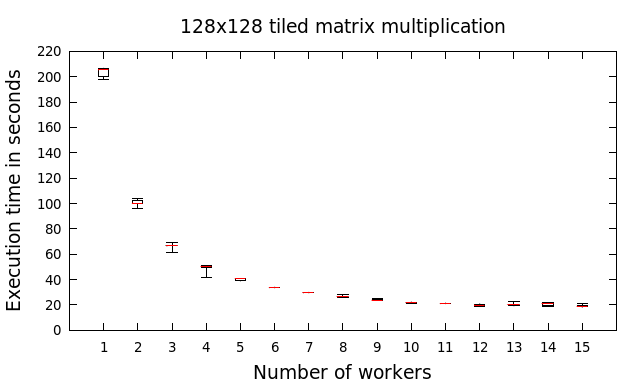
\includegraphics[width=100mm,natwidth=640,natheight=384]{tiledmul_250_100_128x128.png}
%   \caption[TMM execution times for a matrix size of 128$\times$128]{TMM execution times for a matrix size of 128$\times$128}
%   \label{fig:tiledmul_250_100_128x128}
% \end{figure}
% \begin{figure}
%   \centering
%   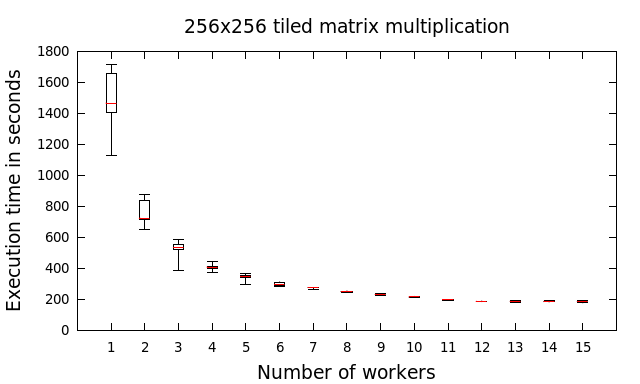
\includegraphics[width=100mm,natwidth=640,natheight=384]{tiledmul_250_100_256x256.png}
%   \caption[TMM execution times for a matrix size of 256$\times$256]{TMM execution times for a matrix size of 256$\times$256}
%   \label{fig:tiledmul_250_100_256x256}
% \end{figure}
% 
% An additional advantage of TMM benchmarks over the ZDT-3 benchmarks is the small amount of data that needs to be transmitted. Like in the ZDT-3 benchmarks, each task data consists of two parents that are sent from the master to the worker, the result is an offspring with its fitness value. In contrast to ZDT-3 --- where an individual consists of a number of \texttt{double} values according to its genome size --- a TMM individual consists of the tile sizes for the $i$, $j$ and $k$ loop. Each of them is a single \texttt{integer} with 4 bytes. The total amount of data that needs to be transmitted from the master to the workers is therefore $2 \times 3 \times 4 \times 25000 = 600000$ bytes or \unit[4.8]{Mb}. Together with the computationally intense tasks of matrix multiplication on the workers (leading to lower network usage) and the absence of time consuming ranking and crowding distance algorithms on the master, this provides speedups of up to 10.507 for 128$\times$128 matrices and 7.961 for 256$\times$256 matrices.
% 
% The reason for the better performance of the 128$\times$128 benchmark over the 256$\times$256 benchmark is unknown. A possible explanation is that the tile sizes are taken from a bigger range (256 instead of 128) which makes it more likely that bad tile sizes are chosen. This is, however, pure speculation.


% \subsection{Speedups}
% Figure \ref{fig:speedup} depicts the speedups for all test problems with respect to increasing worker sizes. The ZDT-3 benchmarks show poor results. This is not surprising as the maximum theoretical speedups of this problem are small (see table \ref{table:theoretical_speedup}) and the communication overhead is bigger compared to TMM. The only unexpected outcome was that the benchmarks scale very bad with a maximum speedup of 2.498 for 1000 genomes. The reason is that the ZDT-3 benchmarks are CPU bound by the master, as the investigations in section \ref{chap:evaluation:result:zdt3} suggest.
% 
% TMM demonstrate better results, the maximum speedup was 10.507 for a matrix size of 128$\times$128. In this case, the speedup grows near linear or even slightly better than linear with the number of workers. That a speedup is better than linear is usually suspicious but can be explained by the fact that each benchmark was repeated five times and the average times of this five executions were taken to compute the speedups. Five executions seem to be too small for getting smooth results, especially when taking into account that the YARN container placement has big influences on the execution times.
% 
% The speedups for the 128$\times$128 TMM increase until a worker size of 12 is reached. At this point, no more improvements are achieved. The reason for this is the limited number of CPUs in the cluster.
% 
% The speedup for the 256$\times$256 TMM benchmark is worse compared to the 128$\times$128 TMM, although it also grows nearly linear until 12 workers.
% 
% \begin{figure}
%   \centering
%   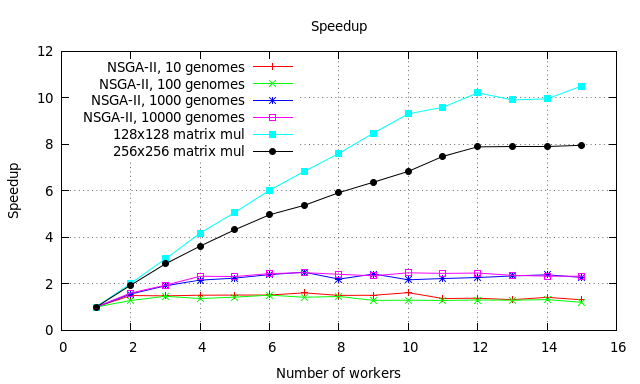
\includegraphics[width=130mm,natwidth=640,natheight=384]{speedup.png}
%   \caption[Speedups for ZDT-3 and TMMs]{Speedups for ZDT-3 and TMMs}
%   \label{fig:speedup}
% \end{figure}





% A good sequential-to-parallel ratio means that the time spent in parallel executable code is high compared to the time spent on code parts that must run sequentially. This is favorable as it brings the potential of higher speedups. It doesn't mean, although, that those speedups can also be reached. This depends on many factors, like the problem itself, the implementation, the environment, etc.
% 
% On the other side, bad sequential-to-parallel execution time ratios mean low achievable speedups. For example, the parallelization of an algorithm with an achievable speedup of 2 can at most halve the execution time of the sequential version, no matter how many resources are used.
% 
% Amdahl's law \cite{amdahl1967validity} is used to compute the achievable speedups for the benchmarks of section \ref{chap:evaluation:testproblems}:
% 
% \begin{equation}
% S = T / (T - t_p)
% \end{equation}
% 
% where $S$ is the achievable speedup, $T$ is the execution time for $SB$ and $t_p$ is the time spent in code parts that can be parallelized. The parallel code parts of the given benchmarks consist of offspring creation and evaluation. Workers execute those parts when the test problems are executed with Biohadoop.
% 
% Table \ref{table:speedup_bounds} shows the results for the achievable speedups. One can see that the ZDT-3 benchmark is not well-suited for parallelization. This is due to the fact that the calculation of the ZDT-3 function is not compute intense. The sequential part of NSGA-II has a large influence on the whole algorithm runtime. This may be different for a more compute intense objective function. The TMM speedup boundaries instead show that TMM is well suited for parallelization.
% 
% \begin{table}
%   \centering
%   \caption{Upper and lower speedup boundaries}
%   \begin{tabular}{lrr}\toprule[2pt]
%     Test Problem & Lower bound & Upper bound \\ \midrule
%     NSGA-II, 10 genomes & 11.923 & 12.568 \\
%     NSGA-II, 100 genomes & 8.025 & 9.640 \\
%     NSGA-II, 1000 genomes & 10.103 & 11.774 \\
%     NSGA-II, 10000 genomes & 11.330 & 11.955 \\
%     TMM, 128$\times$128 & 178.341 & 241.770 \\
%     TMM, 256$\times$256 & 248.950  & 280.542 \\ \bottomrule[2pt]
%   \end{tabular}
%   \label{table:speedup_bounds}
% \end{table}





% The min. and max. sequential execution times of $SB$ are used to compute the true speedups of parallel benchmarks. Table \ref{table:sequential-runtimes} shows the sequential execution time results. One can see that the min. and max. values differ only by a small amount with the exception of TMM with a matrix size of 128x128.
% 
% \begin{table}
%   \centering
%   \caption[Execution times for standalone sequential implementations]{Execution times for $SB$}
%   \begin{tabular}{lrr}\toprule[2pt]
%     Test Problem &  Min. [s] & Max. [s] \\ \midrule
%     NSGA-II, 10 genomes & 2.852 & 3.049 \\
%     NSGA-II, 100 genomes & 2.956 & 3.242 \\
%     NSGA-II, 1000 genomes & 7.673 & 8.865 \\
%     NSGA-II, 10000 genomes & 71.390 & 72.150 \\
%     TMM, 128$\times$128 & 132.066 & 178.639 \\
%     TMM, 256$\times$256 & 1500.705 & 1587.130 \\ \bottomrule[2pt]
%   \end{tabular}
%   \label{table:sequential-runtimes}
% \end{table}
% 
% The difference is due to the nature of the TMM test problem and its objective function. As can be seen in section \ref{chap:evaluation:tiledmul}, the objective is to minimize the execution time of a TMM. A matrix multiplication must be performed to compute the objective function value for a given tile size. The duration of this multiplication depends on the tile sizes. If a benchmark happens to use bad tile sizes often (= long duration for matrix multiplications), its execution time will be higher compared to a benchmark that happens to use good tile sizes (= short duration for matrix multiplications).
% 
% This observed effect is one reason why boundaries are used for the speedup computations. Other effects with even higher influence were identified during the benchmarks. More details about them can be found in section \ref{chap:evaluation:discussion}.





% The $SB$ benchmarks have a second function: the min. and max. sequential execution times of the test problems are used to compute the true speedups of $PB$. Table \ref{table:sequential-runtimes} shows the sequential execution time results. One can see that the min. and max. values differ only by a small amount with the exception of TMM with a matrix size of 128x128.
% 
% \begin{table}
%   \centering
%   \caption[Execution times for standalone sequential implementations]{Execution times for $SB$}
%   \begin{tabular}{lrr}\toprule[2pt]
%     Test Problem &  Min. [s] & Max. [s] \\ \midrule
%     NSGA-II, 10 genomes & 2.852 & 3.049 \\
%     NSGA-II, 100 genomes & 2.956 & 3.242 \\
%     NSGA-II, 1000 genomes & 7.673 & 8.865 \\
%     NSGA-II, 10000 genomes & 71.390 & 72.150 \\
%     TMM, 128$\times$128 & 132.066 & 178.639 \\
%     TMM, 256$\times$256 & 1500.705 & 1587.130 \\ \bottomrule[2pt]
%   \end{tabular}
%   \label{table:sequential-runtimes}
% \end{table}
% 
% The difference is due to the nature of the TMM test problem and its objective function. As can be seen in section \ref{chap:evaluation:tiledmul}, the objective is to minimize the execution time of a TMM. A matrix multiplication must be performed to compute the objective function value for a given tile size. The duration of this multiplication depends on the tile sizes. If a benchmark happens to use bad tile sizes often (= long duration for matrix multiplications), its execution time will be higher compared to a benchmark that happens to use good tile sizes (= short duration for matrix multiplications).
% 
% This observed effect is one reason why boundaries are used for the speedup computations. Other effects with even higher influence were identified during the benchmarks. More details about them can be found in section \ref{chap:evaluation:discussion}.
% 
% \section{Definition of Algorithm Execution Time on Hadoop}
% \label{chap:evaluation:exec-definition}
% The execution time of an algorithm running on top of Biohadoop is composed of the time Biohadoop needs to start up and the algorithm execution time (see figure \ref{fig:execution-times}). The start up begins with Biohadoops submission to Hadoop and ends when the algorithms \texttt{run} method is invoked. The algorithm execution time starts with the invocation of the algorithms \texttt{run} method and ends when this method returns.
% 
% \begin{figure}
%   \centering
%   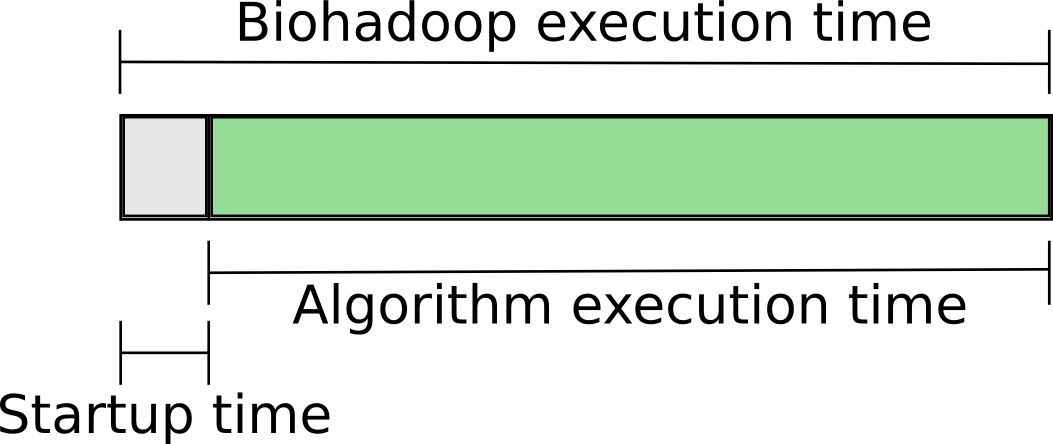
\includegraphics[width=60mm,natwidth=1053,natheight=444]{execution-times.png}
%   \caption[Division of Biohadoop execution times]{Biohadoop execution times are composed of start up times and algorithm execution times}
%   \label{fig:execution-times}
% \end{figure}
% 
% The distinction between start up time and algorithm execution time is made because the main part of the start up time is spent between the application submission to YARN and the beginning of its execution. It is not possible to predict when an application is executed by Hadoop as it depends on different factors like the available cluster resources. To minimize the impact of this uncertainty, the benchmark measurements are based on the algorithm execution time, without the application start up time.